%===================================================================================
% JORNADA CIENTÍFICA ESTUDIANTIL - MATCOM, UH
%===================================================================================
% Esta plantilla ha sido diseñada para ser usada en los artículos de la
% Jornada Científica Estudiantil de MatCom.
%
% Por favor, siga las instrucciones de esta plantilla y rellene en las secciones
% correspondientes.
%
% NOTA: Necesitará el archivo 'jcematcom.sty' en la misma carpeta donde esté este
%       archivo para poder utilizar esta plantila.
%===================================================================================



%===================================================================================
% PREÁMBULO
%-----------------------------------------------------------------------------------
\documentclass[a4paper,10pt,twocolumn]{article}

%===================================================================================
% Paquetes
%-----------------------------------------------------------------------------------
\usepackage{amsmath}
\usepackage{amsfonts}
\usepackage{amssymb}
\usepackage{jcematcom}
\usepackage[utf8]{inputenc}
\usepackage{listings}
\usepackage[pdftex]{hyperref}
\usepackage{caption}
\usepackage{subcaption}
%-----------------------------------------------------------------------------------
% Configuración
%-----------------------------------------------------------------------------------
\hypersetup{colorlinks,%
	    citecolor=black,%
	    filecolor=black,%
	    linkcolor=black,%
	    urlcolor=blue}

%===================================================================================



%===================================================================================
% Presentacion
%-----------------------------------------------------------------------------------
% Título
%-----------------------------------------------------------------------------------
\title{Modelo logístico para el crecimiento poblacional: Capacidad de carga en Cuba entre 1980 y 2020}

%-----------------------------------------------------------------------------------
% Autores
%-----------------------------------------------------------------------------------
\author{\\
\name Autor Guillermo Cepero Garcia \email \href{mailto:thewillyjake53@gmail.com}{thewillyjake53@gmail.com}
	\\ \addr Grupo D111 \AND
\name Luis Ernesto Serras Rimada \email \href{mailto:luisernestoserras@gmail.com}{luisernestoserras@gmail.com}
  \\ \addr Grupo D111}

%-----------------------------------------------------------------------------------
% Tutores
%-----------------------------------------------------------------------------------
\tutors{\\
Lic. Lázaro Daniel González Martínez, \emph{Departamento de Matemática Aplicada.}}

%-----------------------------------------------------------------------------------
% Headings
%-----------------------------------------------------------------------------------
\jcematcomheading{\the\year}{1-2}{Guillermo Cepero Garcia, Luis Ernesto Serras Rimada}

%-----------------------------------------------------------------------------------
\ShortHeadings{Modelo predictivo del crecimiento poblacional}{Autores}
%===================================================================================



%===================================================================================
% DOCUMENTO
%-----------------------------------------------------------------------------------
\begin{document}

%-----------------------------------------------------------------------------------
% NO BORRAR ESTA LINEA!
%-----------------------------------------------------------------------------------
\twocolumn[
%-----------------------------------------------------------------------------------

\maketitle

%===================================================================================
% Resumen y Abstract
%-----------------------------------------------------------------------------------
\selectlanguage{spanish} % Para producir el documento en Español

%-----------------------------------------------------------------------------------
% Resumen en Español
%-----------------------------------------------------------------------------------
\begin{abstract}

	El análisis del crecimiento poblacional reviste gran importancia debido a su relevancia en diversos campos como
	la economía, demografía, epidemiología y la ecología. El objetivo de este trabajo es determinar cuántas personas 
	pueden ser sosteniblemente alojadas en una región, utilizando la capacidad de carga de un modelo logístico ajustado 
	a los datos. El análisis se centró en el crecimiento poblacional cubano desde 1980 hasta 2020, estimando mediante técnicas 
	de mínimos cuadrados la capacidad de carga (K) y la tasa de crecimiento (r) de este modelo. Se proponen diferentes enfoques, 
	incluyendo modelos sin intervalos y con intervalos de 5, 8 y 10 años, para comparar la precisión de los ajustes. Los resultados 
	mostraron que el modelo con intervalos de 8 años fue el de mejor ajuste. El estudio subraya la necesidad de considerar el 
	contexto histórico y los factores específicos de Cuba, como eventos socioeconómicos, al evaluar el crecimiento poblacional. 
	Finalmente, se proponen mejoras al modelo mediante ajustes más detallados y el uso de datos adicionales que incluyan factores económicos y sociales.

\end{abstract}

%-----------------------------------------------------------------------------------
% English Abstract
%-----------------------------------------------------------------------------------
\vspace{0.5cm}

\begin{enabstract}

	The analysis of population growth is of great importance due to its relevance in various fields such as
	economics, demography, epidemiology and ecology. The objective of this work is to determine how many people 
	can be sustainably hosted in a region, using the carrying capacity of a lean logistics model 
	to the data. The analysis focused on Cuban population growth from 1980 to 2020, estimating using techniques 
	least squares the carrying capacity (K) and the growth rate (r) of this model. Different approaches are proposed, 
	including models without intervals and with intervals of 5, 8 and 10 years, to compare the precision of the fits. The results 
	showed that the model with 8-year intervals was the best fitting. The study highlights the need to consider the 
	historical context and Cuba-specific factors, such as socioeconomic events, when evaluating population growth. 
	Finally, improvements to the model are proposed through more detailed adjustments and the use of additional data that include economic and social factors.

\end{enabstract}

%-----------------------------------------------------------------------------------
% Palabras clave
%-----------------------------------------------------------------------------------
\begin{keywords}
	crecimiento poblacional, 
	modelo logístico, 
	capacidad de carga, 
	Cuba
\end{keywords}

%-----------------------------------------------------------------------------------
% Temas
%-----------------------------------------------------------------------------------
\begin{topics}
	Predicción de crecimiento poblacional, estimación del valor de la capacidad de carga.
\end{topics}


%-----------------------------------------------------------------------------------
% NO BORRAR ESTAS LINEAS!
%-----------------------------------------------------------------------------------
\vspace{0.8cm}
]
%-----------------------------------------------------------------------------------


%===================================================================================

%===================================================================================
% Resumen Extendido
%-----------------------------------------------------------------------------------
\section{Resumen Extendido}\label{sec:intro}
%-----------------------------------------------------------------------------------
	El crecimiento poblacional es un fenómeno global que ha tenido un impacto significativo en el desarrollo económico y social de los países. Según las proyecciones de la Organización de las Naciones Unidas para el Desarrollo (ONU), la población mundial alcanzó los 7.9 mil millones en 2021 y se espera que llegue a 9.7 mil millones en 2050 y 11.2 mil millones en 2021. Este crecimiento demográfico tiene implicaciones tanto positivas como negativas para el desarrollo sostenible. Por un lado, el aumento de la población puede generar impulso económico y laboral, especialmente en países con economías en desarrollo. Sin embargo, también plantea desafíos significativos en términos de infraestructura urbana, recursos naturales y servicios públicos\\\\
	El modelo logístico es una ecuación diferencial utilizada para describir el crecimiento poblacional limitado por la capacidad de carga de un entorno. Se basa en la relación entre la tasa de crecimiento y el tamaño de la población en un momento dado. Inicialmente, la población crece de manera exponencial cuando los recursos son abundantes, pero a medida que la población aumenta y los recursos se vuelven limitados, el crecimiento se desacelera y eventualmente se estabiliza al alcanzar la capacidad de carga (K). Matemáticamente se expresa como: $$\frac{dP}{dt} = r \cdot P(t)(1 - \frac{P(t)}{K})$$ \\ donde se tiene que:
	\begin{itemize}
		\item $P(t)$ es la población en función del tiempo $(t)$.
		\item $r$ es la tasa de crecimiento intríseca de la población.
		\item $K$ es la capacidad de carga o tamaño máximo sostenible de la población.
	\end{itemize}
	La solución analítica de la ecuación diferencial es: $$P(t) = \frac{K}{1 + Ae^{-rt}}$$
	donde $A$ es es una constante que depende de las condiciones iniciales de la población (la ecuación para encontrar $A$ es: $P(0) = \frac{K}{1 + Ae^{0}}$). Por lo tanto para describir el crecimiento poblacional en Cuba desde 1980 hasta 2020, se propone realizar un ajuste de parámetros de esta ecuación ($P(t)$) con los datos reales de la población.\\
	Para ello se utiliza la aproximación por mínimos cuadrados por medio de la función curve-fit del módulo scipy.optimize en Python, cuya función matemáticamente se puede representar como:\\
	Minimizar: $\sum_{i=1}^{N} (y_{i} - f(x_{i}, \theta))^{2} $ \\
	donde toma los parámetros:
	\begin{itemize}
		\item f: es la función modelo para la optimización.
		\item xdata: son los valores independientes (el tiempo ($t$ como $x_{i}$)).
		\item ydata: son los valores dependientes (los valores de densidad poblacional en función del tiempo ($P$ como $y_{i}$)).
		\item p0: Estimación inicial.
	\end{itemize}
	\small{La función curvefit intentará minimizar la suma de los cuadrados de los residuales para encontrar los valores óptimos de $K$ y $r$ que minimizan esta expresión.} \\\\	
	Se realiza el desarrollo por medio de dos modelos diferentes, uno sin intervalos de 5,8 y 10 años donde el modelo sin intervalos tuvo un ajuste adecuado \\(\textbf{Ver en Figure 1.}) pero el de intervalos de 8 años fue el que mejor aproximó (\textbf{Ver en Figure 2})  
	\begin{figure}[h!]%
		\begin{center}
			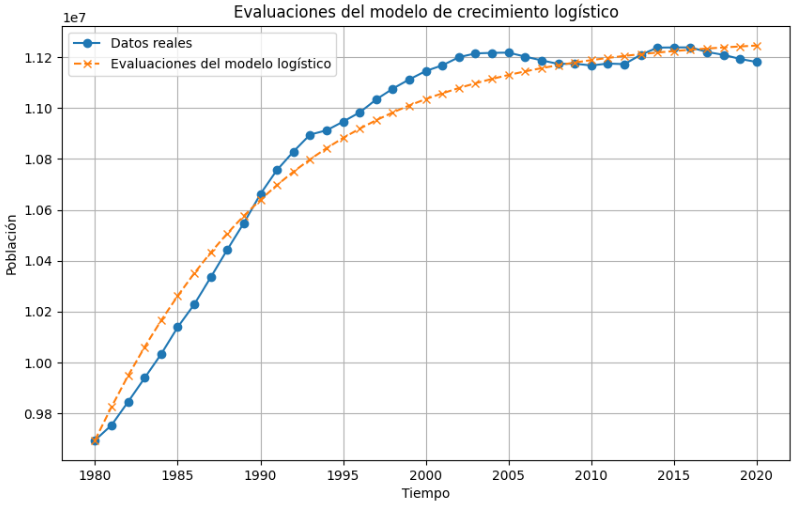
\includegraphics[width=0.45\textwidth]{real_vs_pred.png}
			\caption{Evaluaciones del modelo logístico sin intervalos\label{fig:ex}}
		\end{center}
	\end{figure}

	\begin{figure}[h!]%
		\begin{center}
			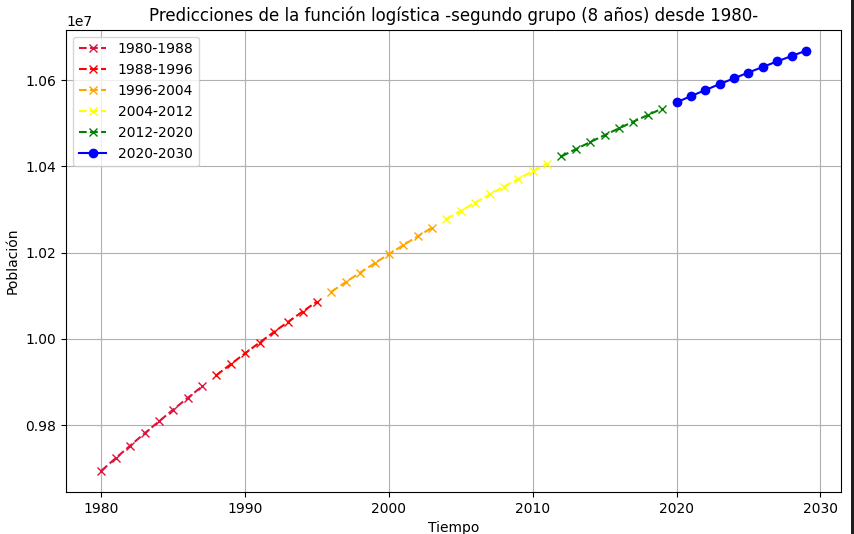
\includegraphics[width=0.45\textwidth]{prediccion.png}
			\caption{Evaluaciones del modelo logístico en intervalos de 8 años\label{fig:ex}}
		\end{center}
	\end{figure}
	\section{Recomendaciones}\label{sec:outro}	
	\normalsize{En busqueda de fortalecer el modelo actual, ampliar su alcance y utilidad, y contribuir al conocimiento demográfico de Cuba, teniendo en cuenta las particularidades observadas en el análisis inicial se propone desarrollar un modelo matemático avanzado para entender mejor el crecimiento poblacional en Cuba, incorporando factores económicos, sociales y políticos, y utilizando técnicas de modelado dinámico. Esto incluye ajustar el modelo a periodos de crecimiento acelerado, ampliar la base de datos con información sobre migraciones, distribución geográfica e indicadores socioeconómicos, así como validar el modelo mediante pruebas comparativas y/o hacer una predicción de cómo se comportará la población cubana en futuros años. Además, se sugiere investigar el impacto de eventos macroeconómicos y factores ambientales en la población. Finalmente, se busca divulgar los resultados en foros académicos y sugerir aplicaciones prácticas para la planificación urbana y políticas públicas, contribuyendo así al conocimiento demográfico del país.}
\end{document}